\subsection{Runtime Calibration} \label{sec:calibration}

As described in Section~\ref{sec:runtime_tuning}, RAT distinguishes known, also called seen, and unknown, also called unseen, rts's.
Known rts's have been encountered during DTA.
Based on the used plugin and optimization criteria, optimal configurations for these are saved in the ATM.
Unknown rts's, however, describe rts which have not been encountered during DTA.
There are several reasons why unseen rts's might occur.
The region itself might be known, but some parameters (e.g., application inputs) changed between DTA and runtime.
Alternatively, an unseen rts could consist of entirely new regions, which were not seen during DTA.
The goal of the runtime calibration is to handle these unknown rts's during RAT.

Since runtime calibration is done during production runs, there are two restrictions for the algorithm:
First, there can be no user input and second, a suitable configuration has to be found in a short time.
Based on these, we implemented a Q-Learning based mechanism, which we introduced in~\cite{Gocht2019a}.
For any unknown rts, the algorithm starts at a given core and uncore frequency.
With a probability of {$\epsilon$}, the algorithm selects a different configuration from the next direct neighbors.
To validate the outcome of the possible optimization, it measures the energy for all configurations.
Based on the result of the measurement, it calculates the so-called Q-Value.
Afterwards, the algorithm chooses the next optimal status according to the Q-Value and starts from the beginning.
Figure~\ref{fig:qlearning} shows how the mechanism searches for an energy-efficient optimum.
It starts an initial setting, with a core frequency of 1.9 GHz and an uncore frequency of 2.2 GHz
When the application terminates, a core frequency of 2.3 GHz and uncore frequency of 2.2 GHz is reached.

\begin{figure}[!t]
\centering
%\includegraphics[trim={7cm 2cm 5.5cm 2cm},clip,width=3in]{readex-approach}
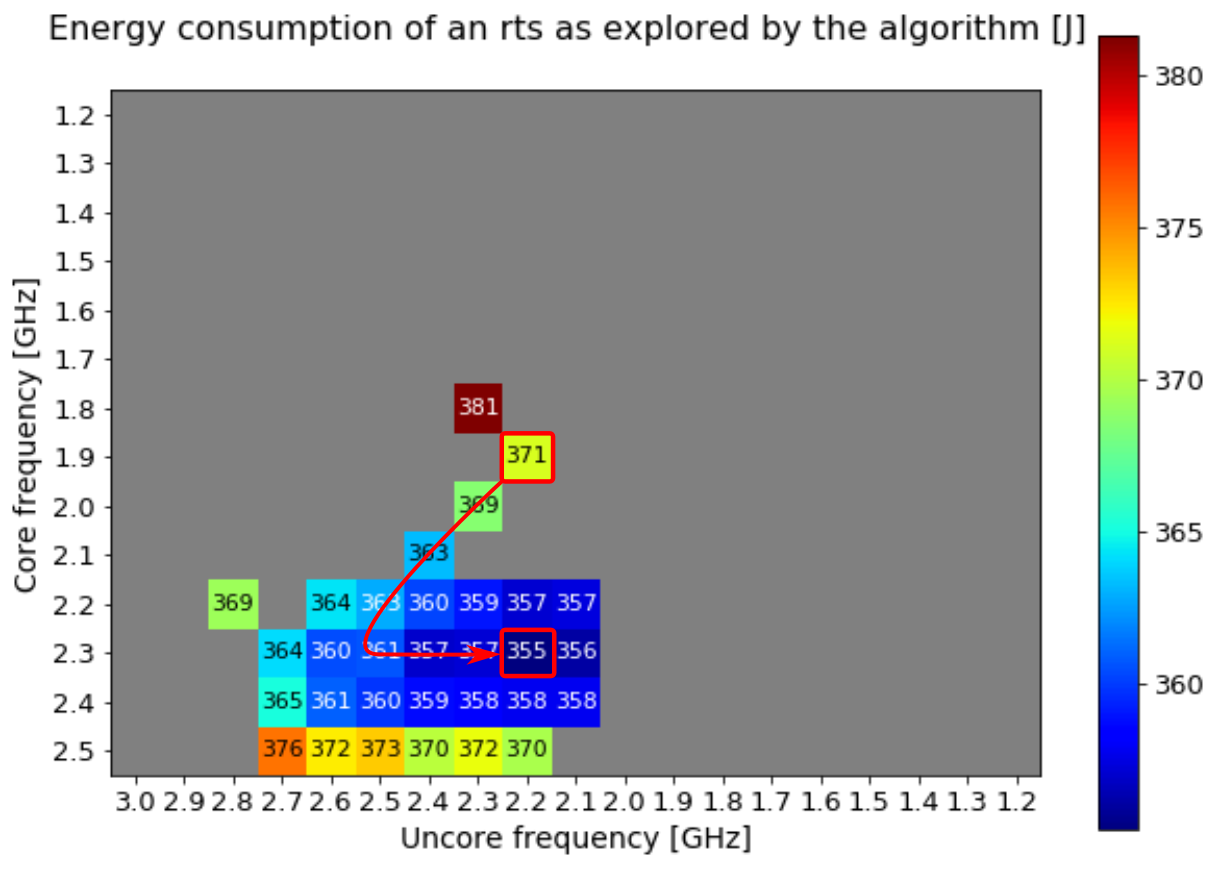
\includegraphics[width=.8\columnwidth]{figures/q_learning.png}
\caption{Heatmap of the energy consumption of a specific region for different core and uncore frequencies as explored by a Q-Learning algorithm applied at runtime.
The algorithm starts at \{1.9, 2.2\} GHz and finds a more suitable setting \{2.3, 2.2\} GHz.}
\label{fig:qlearning}
\end{figure}

% In the second approach, the RRL uses performance counters to predict the optimal setting using neural networks.
% First, the approach identifies the most relevant performance counters.
% In a second step, it trains a shallow neural network in order to predict a good frequency.
% This model is then loaded during runtime.
% Once the RRL encounters an unseen RTS, it measures the relevant performance counters and uses the neural network to predict a good setting.
% In contrast to the Q-Learning approach, this approach does require a pre-training, which has to be performed once per system.
% However, once this is done, the network just needs to be evaluated, which requires less tuning and runtime overhead compared to the Q-Learning approach.
% 
